\section{Experiments}
\label{expall}


\noindent\textbf{Classroom Interaction Database.} As mentioned, we have collected and annotated a database of 100 video clips capturing students' behaviors in interactive class sessions. The students are seated but occasionally engaged into small-group discussions. The groups are formed in an ad-hoc manner and vary in geometric configurations. The 15 fps videos come from five cameras covering different areas of a lecture hall, the lengths of them vary from one minute to four minutes, and the numbers of individuals in the video varies from six to twenty. See Figure \ref{diagram} for example frames. We have applied an OpenCV face detector to the videos, and generated long tracks of the bounding boxes using a combination of OpenCV mean-shift tracking and dominant optical flows in the bounding boxes. We manually eliminate the false-alarm boxes/tracks and recover (very few) miss-detections when using the video for building ground-truth exemplars, and do not involve manual correction when testing our approach. In each video, we have manually identified the participants of all two-person, three-person, and four-person interactions as well as their exact occurrence intervals. Totally, 254 two-person, 112 three-person, and 16 four-person interactions are annotated from all videos. In consultation with education experts, we further divide the two-person interactions into three categories (same row, left-back row v.s. right front row, right-back-row v.s. left-front row), and the three-person interactions into four categories (three people in the same row with two looking left, three people in the same row with two looking right, two people in the back row, two people in the front row)\footnote{It is observed by education experts that students' relative pose and positions strongly modulate their behaviors (\textit{e.g.} see \cite{Crouch:PI}) and consequently under their guidance we categorize the interactions based on students' relative pose and geometric configurations.}. Examples of these patterns are shown in Figure \ref{dataset}. The lengths of these occurrence intervals, meanwhile, range from a few seconds to tens of seconds. The 100 videos arise from five long-lectures, and we adopt a leave-one-lecture-out scheme in partitioning the training (database) exemplars and testing (input) videos. A separate dissimilarity measure is trained from each camera.


\begin{figure}[t]
\begin{center}
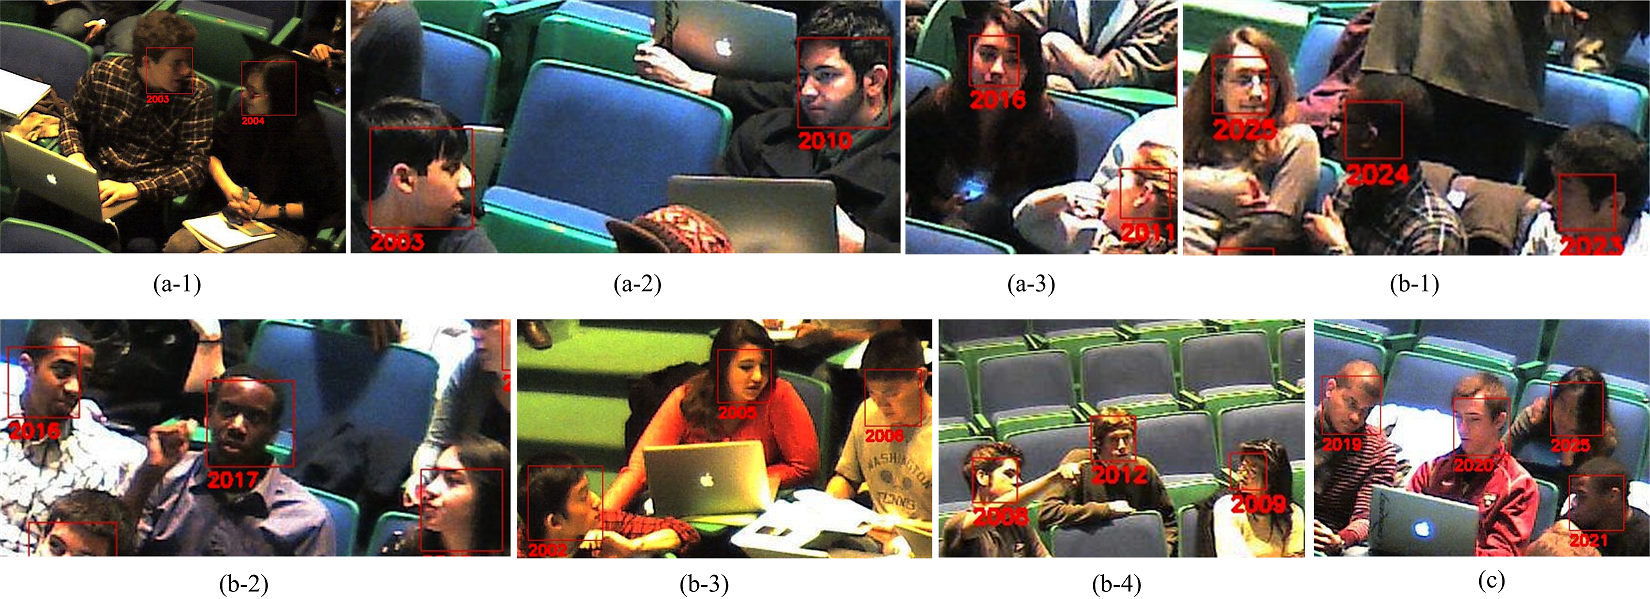
\includegraphics[scale=1.2]{dataset.png}
\end{center}
\caption{Samples of two-person ((a-1)(a-2)(a-3)), three-person ((b-1)(b-2)(b-3)(b-4)), and four-person (c) interactions in the classroom interaction dataset we collected.}
\label{dataset}
\end{figure}



A 4-level pyramid is set up at each ground-truth time interval, and a temporal unit is set at half length of the bottom-level cell. We use a coarse representation of the head pose as the individual activity descriptor. Specifically, we apply local translational alignment and size normalization to the bounding boxes with adjacent frames to compensate for imperfect tracking. Then, we compute the Histogram of Oriented Gradient (HOG) feature within each temporal unit and each box, and apply nine one-against-all SVMs to estimate the likelihood of a HOG feature belonging to nine head poses (front, left, lower-left, lower-front, lower-right, right, back-right, and back-left). The nine-dimensional likelihood vector eventually serves as our individual activity descriptor. On the other side, we derive the contextual descriptor for three or more individuals based on the geometrical configurations of the bounding boxes. As shown in the left panel of Figure \ref{all_illu}(b), where a descriptor of human $m$ in context of human $m'$ among five humans at time $t$ is computed, we compute the distances $r_{i}$'s between all others and $m$, and the relative angles $a_{i}$'s between the connecting vectors and $\overrightarrow{mm'}$, and combine all these geometric quantities into a contextual descriptor $\mathbf{g}_{m,m',t}$. When computing $\mathbf{g}_{n,n',s}$ in the input (right panel of Figure \ref{all_illu}(b)), we align $\overrightarrow{nn'}$ against $\overrightarrow{mm'}$ and predict the locations of the three individuals (shown in red), and compute the true distances $z_{i}$'s and relative angles $b_{i}$'s by locating the nearest individuals to the predicted locations. This contextual representation achieves invariance under similarity transforms. For two-person interaction, we simply use the distance and the relative angles against the right horizontal axis (Figure \ref{all_illu}(c)). 

\begin{table}[ht]
\centering \caption{Computational cost comparison for the proposed matching approach and baselines (in seconds).}
\footnotesize{
\begin{tabular}{|c|c|c|c|}
\hline    \# of Participants &  2  &  3  &  4   \\
\hline   Exhaustive+Sliding Window & 17.2   & 60.4   & 253.2   \\
\hline  Exhaustive+Branch and Bound &  12.6 &  27.6  &   59.7 \\
\hline  Optimal Pairing+Sliding Window & 12.4  & 23.2   &  40.8  \\
\hline  Proposed & 8.0  &  19.8  &  32.3  \\
\hline 
\end{tabular}
}
\label{computecost}
\end{table}


Before we look into the performance in correct detection and classification, we first look into the computational cost of the approach. We replace the optimal matching method with an exhaustive enumeration of all possible matchings. We also apply temporal sliding windows at different scales, and stop using the remaining scales whenever the current window achieves the same quality function value as the branch-and-bound, but we try at most eight scales ranging from half to twice of the exemplar length. We show the average computation time for one match between an exemplar and an input on a 8-core 2.8GHz Macintosh in Table \ref{computecost}, where we see clear savings for the proposed approach.


\begin{figure*}[t]
\begin{center}
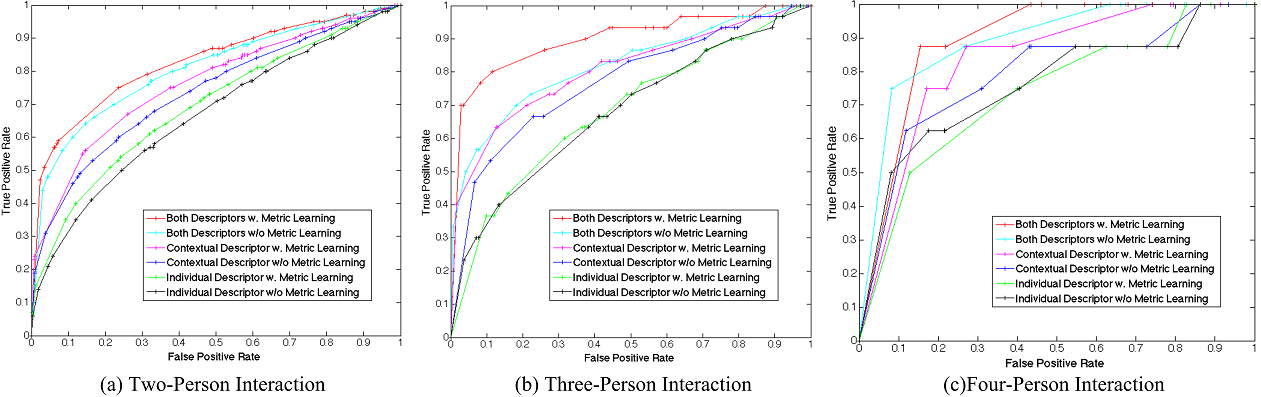
\includegraphics[scale=2.5]{ROC.png}
\end{center}
\caption{ROC curves for identifying the participants of an two-person, three-person, and four-person interactions using the proposed approach and baselines. }
\label{ROC}
\end{figure*}

Note that we combine both individual activity (pose) descriptor and interaction (geometric context) descriptor and learn an optimal dissimilarity, we then evaluate the effect of this combination by using either descriptor (but not both) and identity matrices as the dissimilarity parameter. The ROC curves for detecting the participants of an interaction is shown in Figure \ref{ROC}. Note that using both descriptors and learning the optimal dissimilarity do yield the best performance, while it is interesting to see that contextual descriptor performs better than individual descriptor, mainly due to the fact that the interaction only occur among nearby students in a classroom environment and therefore geometric context provides a strong clue for a potential occurrence of interaction. Also note that increased number of participants achieves higher true positives against false positives. This phenomenon is expected, as when more contextual information is available from more humans, the true interaction pattern is more discriminative against the false ones.

\begin{figure*}[t]
\begin{center}
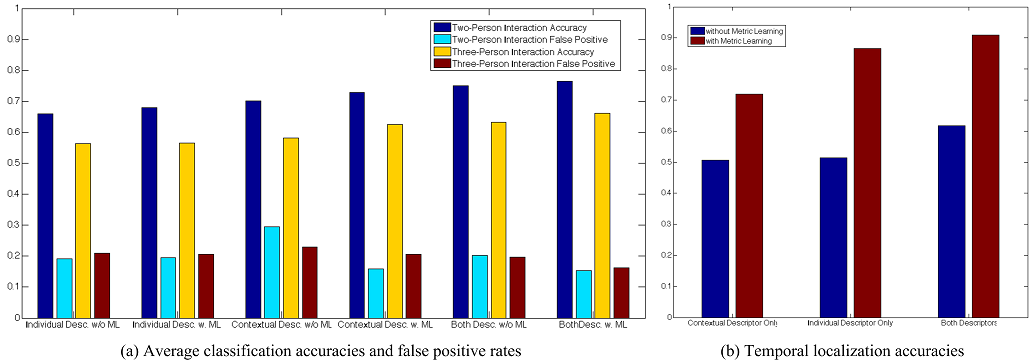
\includegraphics[scale=2.5]{classtemporal.png}
\end{center}
\caption{ Average classification accuracies and false positives for two-person and three-person interactions (Individual and/or contextual descriptors, with or without metric learning (ML)) and the temporal localization accuracies.}
\label{classtemporal}
\end{figure*}

The third evaluation is on the classification performance for the two-person and three-person interactions (as no further categorization for the four-person interactions is provided, no classification results on four-person interactions are shown). We examine those correctly detected pairs and triples and show the average true positive rates v.s. false positives when further classifying them into the three or four categories in Figure \ref{classtemporal}(a). Again note that either the dissimilarity learning or combining both descriptors gives rise to moderately improvement. As we are  at this stage investigating the correctly identified pairs or triples, the head poses serves a stronger evidence than spatial configuration for classification. A pose estimator, which is improved from current coarse representation and is more robust to videos of limited quality, will expect further improved classification performance.


We finally investigate the temporal localization performance. For this purpose, we compute the ratio of the intersection to the union of the estimated interval and the annotated interval, and show the averages in Figure \ref{classtemporal}(b).  Note that the dissimilarity learning is designed in such a way as to encourage the group dissimilarity function to achieves negatives within an activity and positives otherwise. Therefore, the learned quality function of the branch-and-bound search more precisely reflects the boundaries of an activity.


\begin{figure*}
\begin{center}
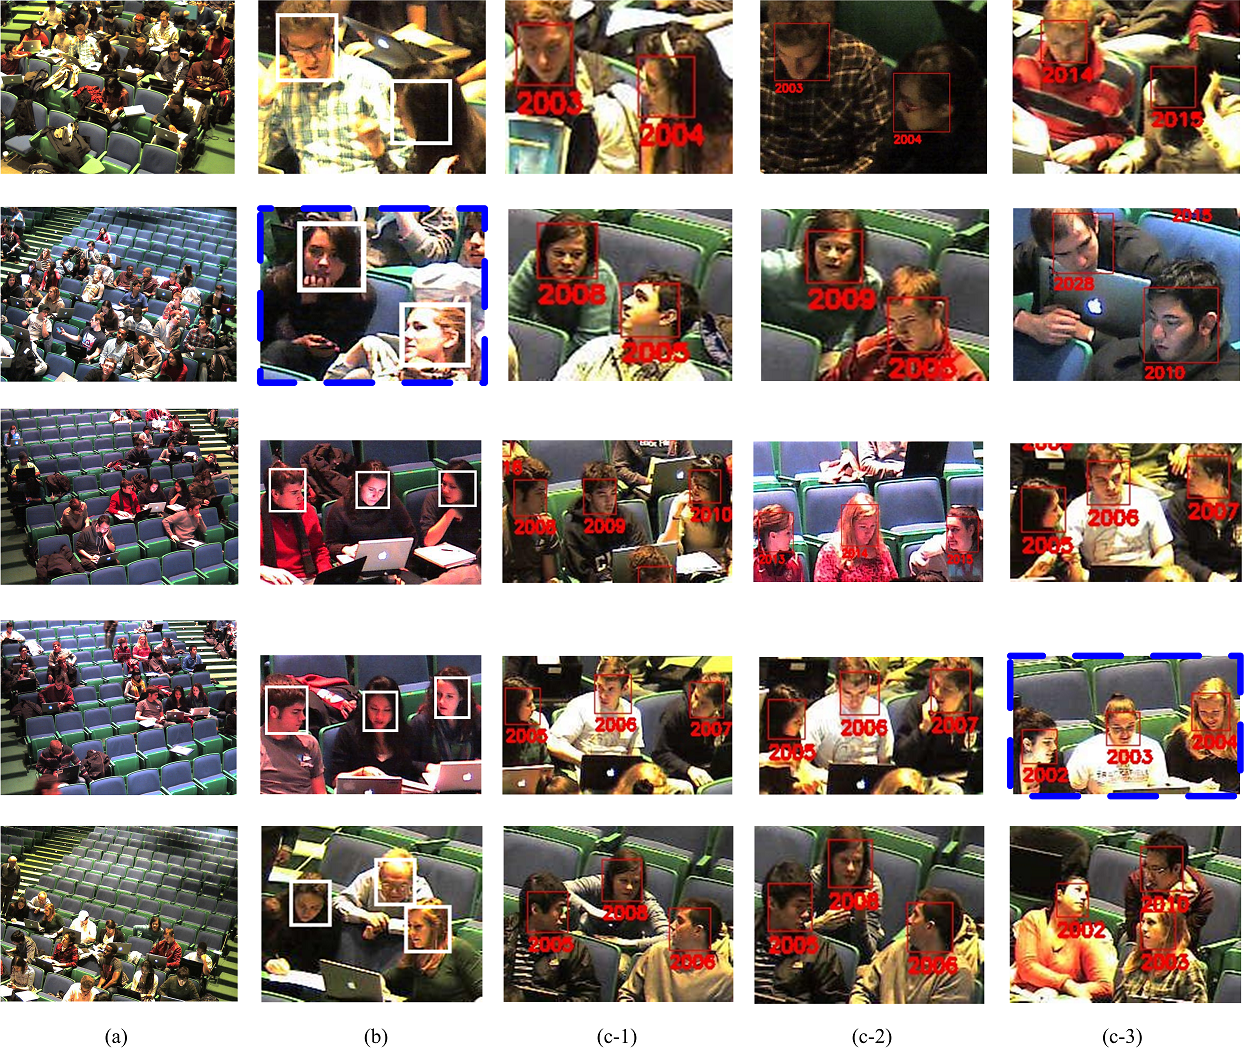
\includegraphics[scale=2.25]{retrieved.png}
\end{center}
\vspace{-10pt}
\caption{Examples of social interaction detection and matching on the classroom interaction database. Each row is an example of detecting a salient interaction from an input and enumerating similar database exemplars: (a) is the input, (b) is the detected social interaction, and (c-1) to (c-3) are the top three associated database exemplars that support this detection.}
\label{retrieved}
\end{figure*}


As a visualization, Figure \ref{retrieved} shows examples of group interaction detection and matching on the classroom interaction database. Note that in the first and third row, a two-person interaction and a three-person interaction are correctly detected and associated with correct exemplars. In the second row, a false positive is detected (shown in blue dashed box), in which the two people are not interacting but demonstrating head poses that are similar to those in a conversation. In the fourth row, the three-person interaction (two looking to the left) is correctly detected but supported by an exemplar of different category (shown in blue dashed box, annotated as `two looking to the right'). Note that the head pose of person marked `2003' appears ambiguous between `looking to the left' and `looking to the right'. In the fifth row, a three-person interaction is correctly identified and associated with correct exemplars, though the head poses of the participants moderately vary among exemplars. 

\vspace{0.05in}
